
The microbiome temporal variability was analyzed to extract the global properties of the system. As fluctuations in total counts are plagued by systematic errors we worked on the temporal variability of relative abundances for each taxon. Our first finding was that, in all cases, changes in the relative abundances of taxa followed a ubiquitous pattern, known as the fluctuation scaling law\cite{fs} or Taylor's power law\cite{taylor}, i.e., the microbiota of all detected taxa followed $\sigma_i  = V\cdot x_i^{\beta}$, a power law dependence between the mean relative abundance $x_i$ and the dispersion $\sigma_i$. The law seem to be ubiquitous, spanning even to six orders of magnitude in the observed relative abundances. As shown in Figure \ref{fig:main1}, the most abundant species were less volatile in relative terms than those which were less abundant. The fitting to the power law was always robust ($R^{2}$ > 0.88) and did not depend on the microbiome condition. The power law (or scaling) index $\beta$ and the variability $V$ (hereafter Taylor's parameters) appear to be correlated with the stability of the community. On the one hand, $\beta$ is a scaling index that gave us information about the statistical properties of the ecosystem. If it is $1/2$, the system behaves like a Poisson distribution. If $\beta$ is 1, the system behaves as an exponential distribution. Generally speaking, metagenomes vary with time with $\beta$ between these two universal classes. In our case, the fact that $\beta$ was less than 1 tells us that the most abundant taxa in the microbial community were less susceptible to any perturbation than the other taxa. On the other hand, the variability $V$ was a direct estimator of the amplitude of fluctuations over time. $V$ represents the maximum variability attainable by a hypothetical dominant genus (with relative abundance close to 1). It is an important parameter that characterizes the type of system. If $V$ is small the ranking is stable such as, for example, the number of diagnoses of a particular disease recorded in Medicare during a month. If $V$ is large, as it seems to be the case of metagenomic samples, the ranking might be unstable, like the number of hourly page views of articles in Wikipedia \cite{ranking,fs}. The Taylor parameters were related to the health status of the host, which we consider as constituting the main finding contributed by this article.

\begin{figure}
	\centering
	\vspace*{-15mm} % Corrects overbox of the figures
	%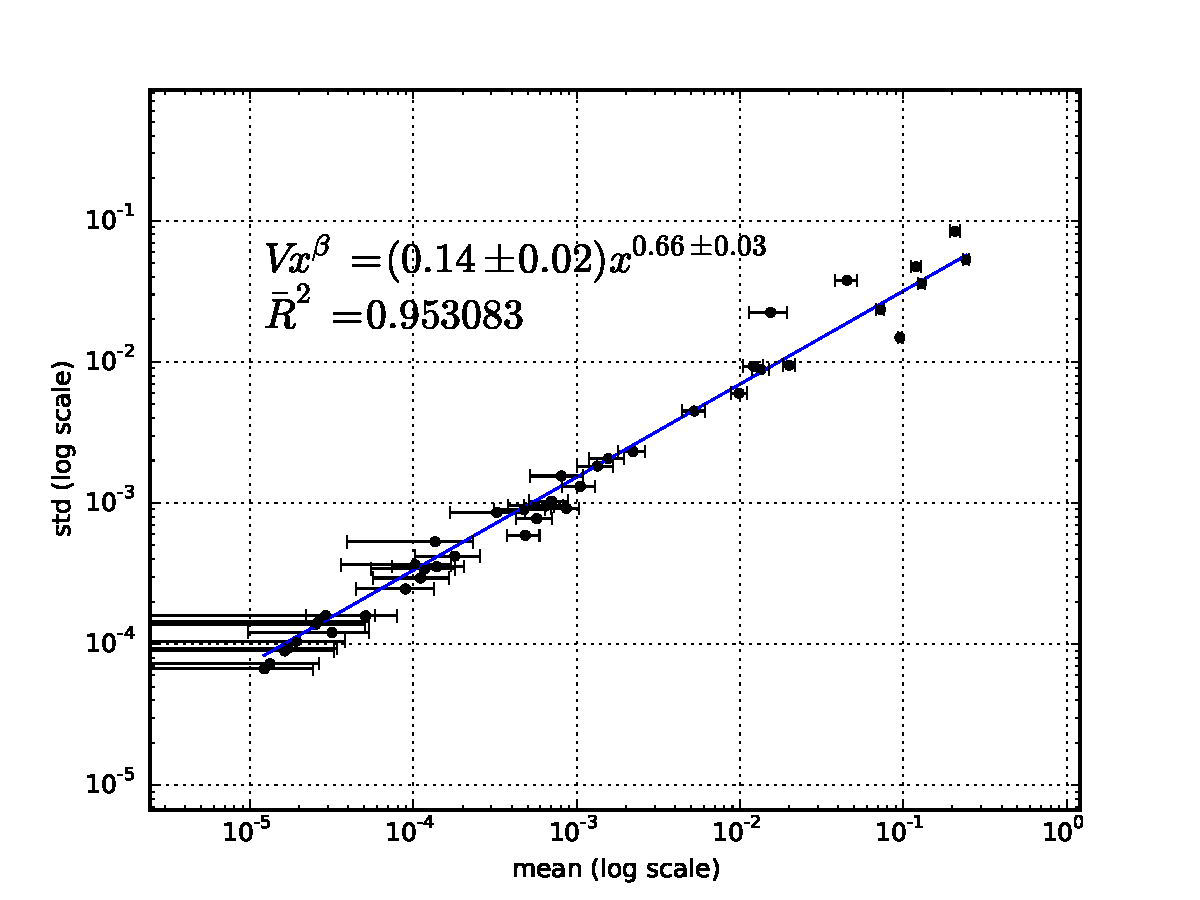
\includegraphics[width=0.8\textwidth]{results/fits/IBS_h_A_amplicons_family_stdVSmean_xWboot_LOG.pdf}
	%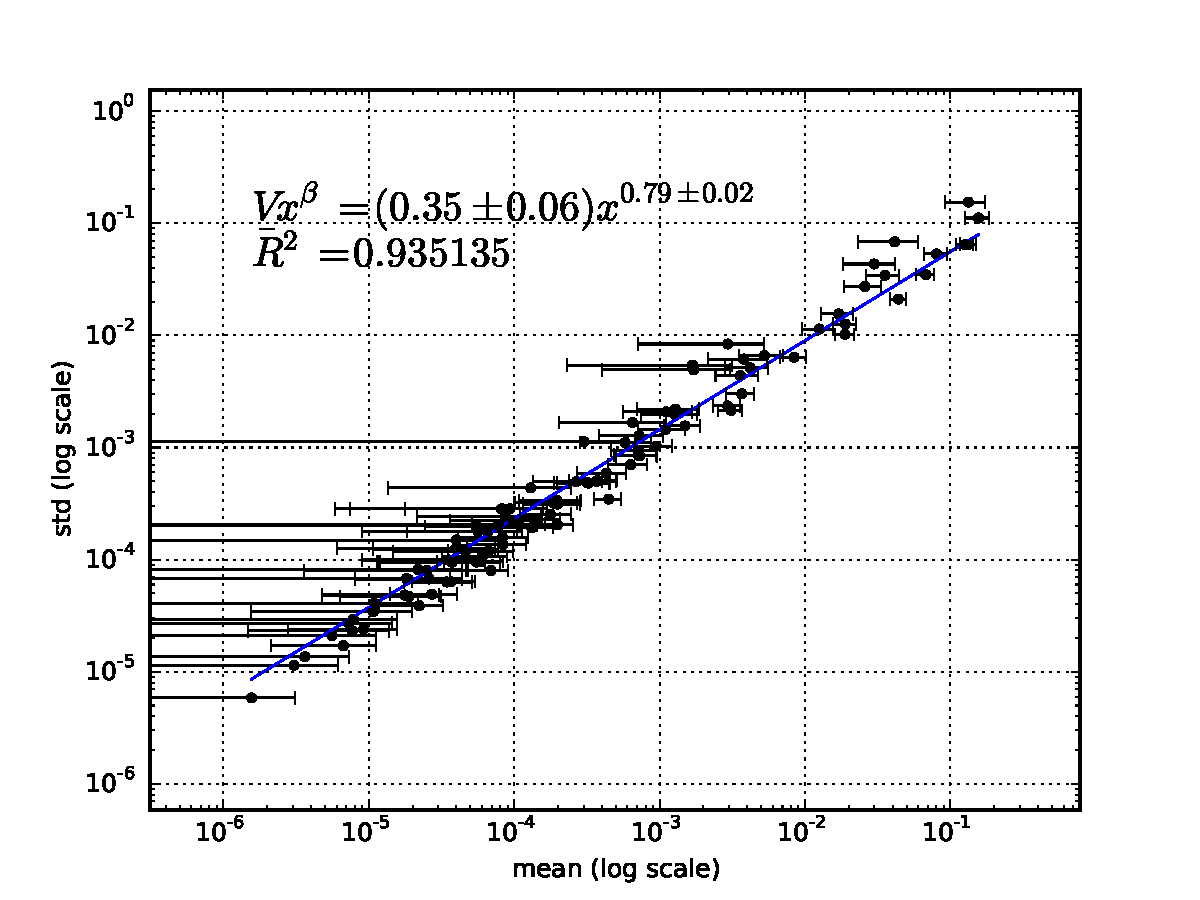
\includegraphics[width=0.8\textwidth]{results/fits/IBS_P2_Metatranscriptores_stdVSmean_xWboot_LOG.pdf}
	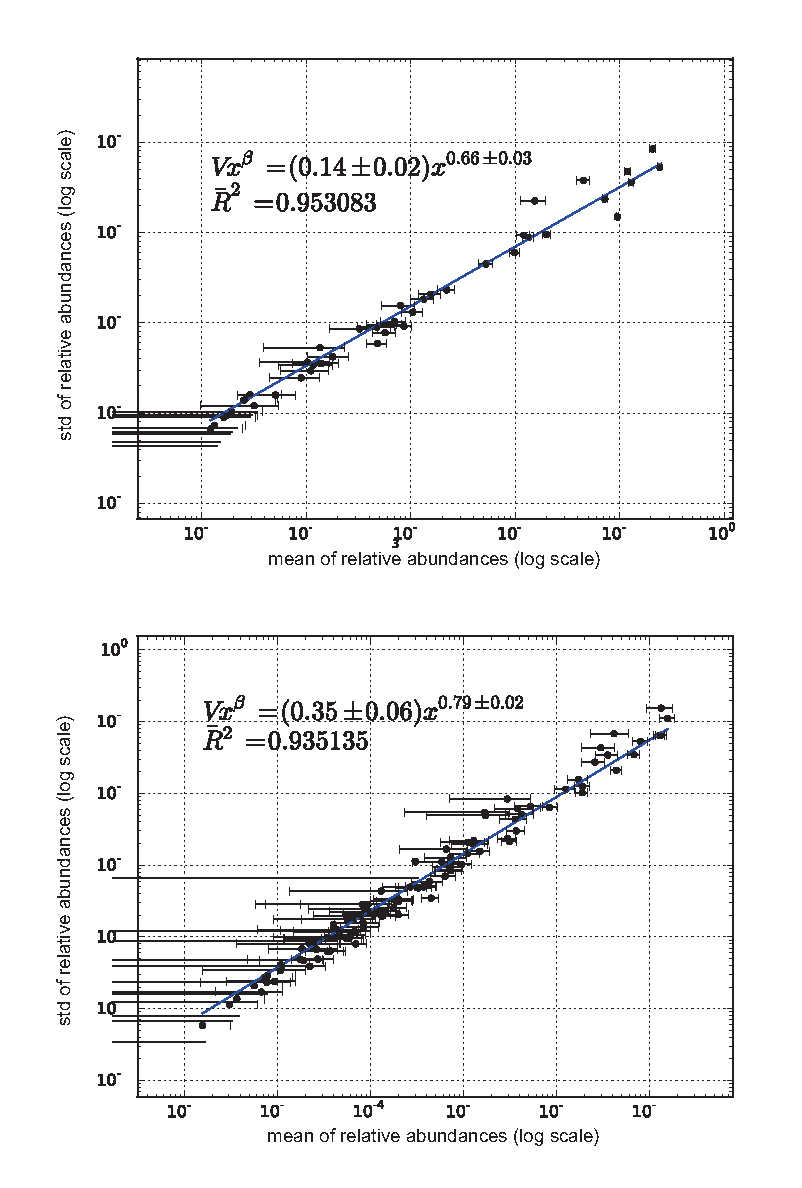
\includegraphics[width=0.8\textwidth]{figs/Fig1.eps}
	\caption{X-weighted power-law fits of the standard deviations versus the mean values for each bacterial genus monitored over time. The fit is shown for samples from a healthy subject (top) and from a subject diagnosed with irritable bowel syndrome (bottom), studied in our lab \cite{IBS}. Taylor's power law seems to be ubiquitous, spanning to six orders of magnitude. The error bars (\emph{mean-axis}) are the SEM.}
	\label{fig:main1}
\end{figure}

Taylor's parameters describing the temporal variability of the gut microbiome in our sampled individuals are shown in Supplementary Tables S\ref{tab:diet} to S\ref{tab:LEA}. Our results hint at ubiquitous behavior. Firstly, the variability (which corresponds to the maximum amplitude of fluctuations) was large, which suggests the resilient capacity of the microbiota. Secondly, the scaling index was always smaller than one, which means that more abundant taxa were less volatile than less abundant ones. In addition, Taylor's parameters for the microbiome of healthy individuals in different studies were compatible with estimated errors. This enabled us to define an area in the Taylor parameter space that we called the \emph{healthy zone}. 

In order to jointly visualize and compare the results of individuals from different studies\cite{IBS,moving,antibiotic,LEA,kwashiorkor,diet,hostlife}, their Taylor parameters were standardized, with standardization meaning that each parameter was subtracted by the mean value and divided by the standard deviation of the group of healthy individuals for every single study independently. Due to the different systematics in each study, we defined a healthy region for each one of them, standardized to mean zero and variance one and computed mean and variance of ?unhealthy? with this standardization (for details of the procedure, please see Standardization subsection in Material and Methods). Therefore, different studies were isolated so that individuals from a given study did not affect the results on the ?unhealthy? individuals of the other studies. We think this statistical approach was safer, as we avoided to combine data with very different systematic errors. The healthy zone and the standardized Taylor parameters for individuals whose gut microbiota was compromised (i.e., they were suffering from IBS, kwashiorkor, altered diet, intake of antibiotics, a Salmonella infection, or had gone on a trip abroad) are shown in Figure \ref{fig:main2}. The variability in children developing kwashiorkor was smaller than that of their healthy twins. A meat/fish-based diet significantly increased variability when compared to a plant-based diet. All other cases presented increased variability, which was particularly severe and statistically significant at over 95\% confidence level (CL), for grade III obese patients on a diet, individuals taking antibiotics, the subject who had a Salmonella infection, the subject who did a travel abroad or the IBS-diagnosed patients. One global property emerged from all the worldwide data collected: the Taylor's parameters characterized the statistical behavior of microbiome changes. Furthermore, we verified that our conclusions were robust to systematic errors as a result of taxonomic assignment (see Taxa level selection in Material and Methods).

\begin{figure}
	\centering
	%\includegraphics[width=0.9\textwidth]{results/finalplot11.pdf}
	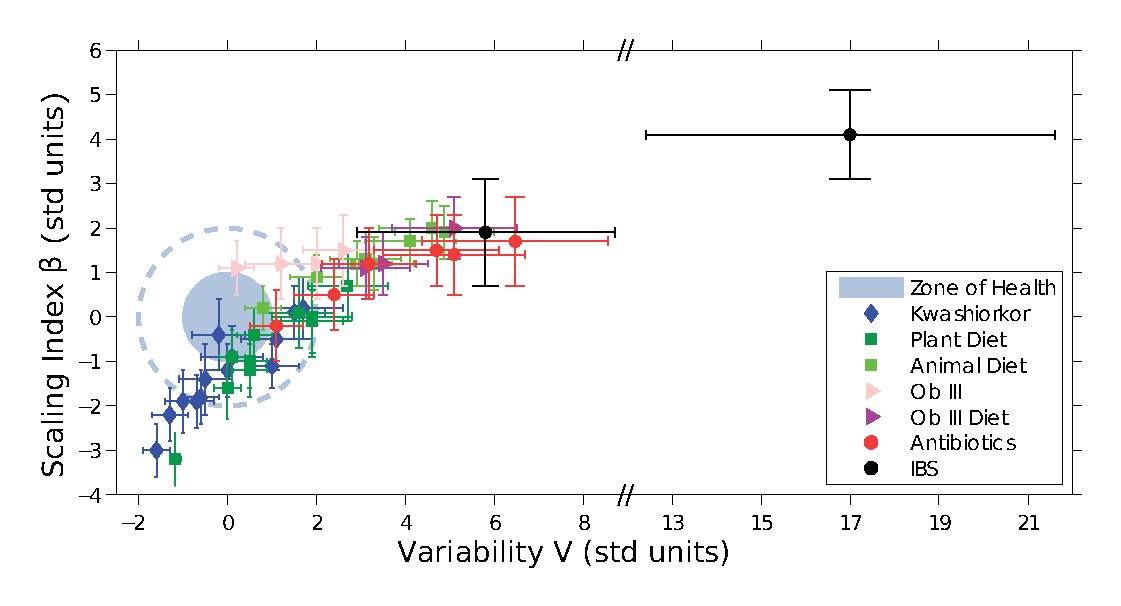
\includegraphics[width=1.0\textwidth]{figs/Fig2.eps}
	\caption{Taylor's law parameter space. All the data studied in this work were compiled here. The colored circle corresponds to a 68\% confidence level (CL) region of healthy individuals in the Taylor's parameter space, while the dashed line delimites the 98\% CL region. Points with errors place gut microbiome in the Taylor's parameter space, for each individual whose microbiota was compromised. It should be noted that the parameters were standardized (standard deviation units) to the healthy group in each study for every single study independently, for demonstrative and comparative purposes.}
	\label{fig:main2}
\end{figure}

Taylor's power law has been explained in terms of various effects, though none have brought a general consensus. It can be shown to have its origin in mathematical convergence which is similar to the central limit theorem, and thus virtually any statistical model designed to produce a Taylor law converges to a Tweedie distribution\cite{stat}, providing a mechanistic explanation based on the statistical theory of errors\cite{convergence1,convergence2,convergence3}. To reveal the generic mechanisms that drive different scenarios in the $\beta-V$ space, we modeled the system by assuming that taxon relative abundance followed a Langevin equation with, on the one hand, a deterministic term that captured the fitness of each taxon and, on the other hand, a randomness term associated with Gaussian random noise\cite{ranking}.Both terms were modeled by power laws, with coefficients that can be interpreted as the taxon fitness $F_i$ and the variability $V$ (see Model in Material and Methods). Fitness $F_i$ captures the time scale that the system needs to reach equilibrium (the size of variability $V$ may or may not allow to reach it). $F_i$ has dimensions of 1/time and roughly corresponds to the half-life of the system when decaying to the stable state. In fact, it is exactly the half-life if $\beta$ is one and $V$ is negligible. In this model, when $V$ is sufficiently low, abundances are stable in time. Differences in the variability $V$ can induce a noise-induced phase transition in the relative abundances of taxa. The temporal evolution of the probability of a taxon having the abundance $x_i$, given its fitness, is governed by the Fokker--Planck equation. The results of solving this equation show that stability is best captured by a phase space determined by the fitness $F$ and the amplitude of fluctuations $V$ (see Figure \ref{fig:main3}).

\begin{figure}
	\centering
	\vspace*{-5mm} % Corrects overbox of the figures
	%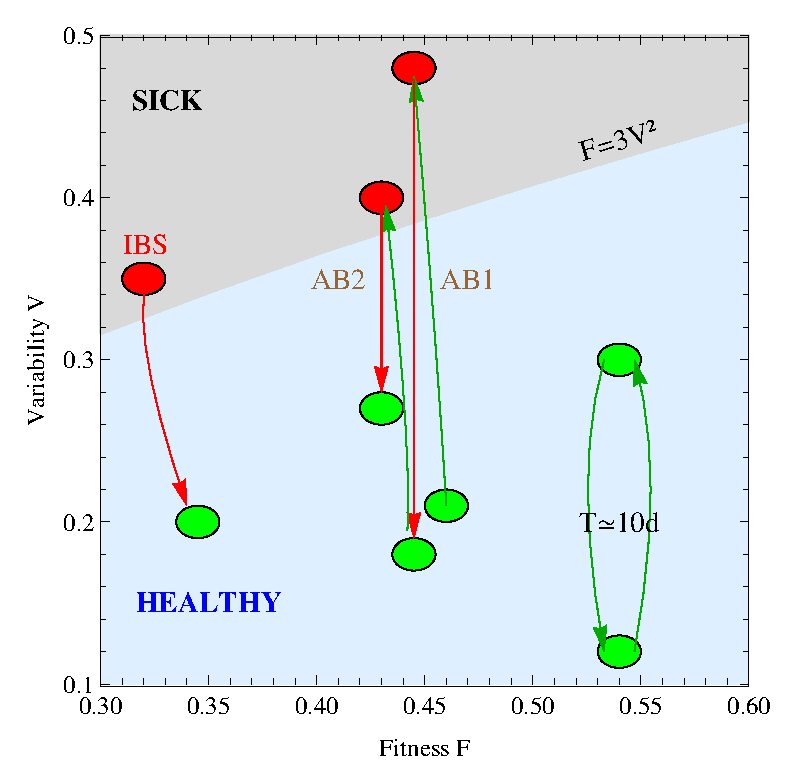
\includegraphics[width=0.8\textwidth]{results/finalPlot33_new.pdf}
	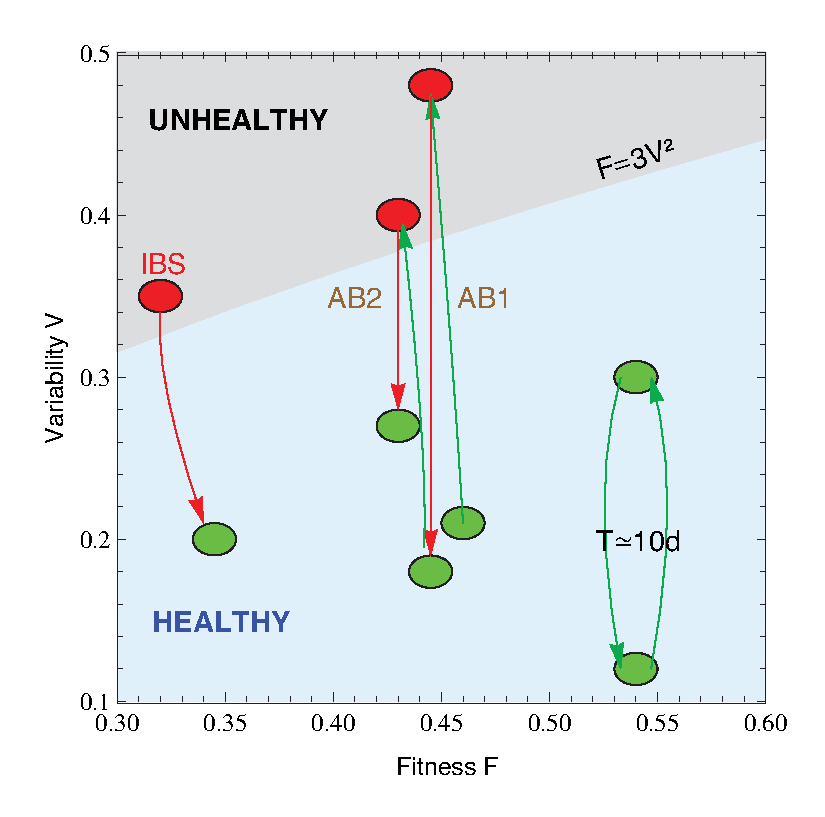
\includegraphics[width=0.8\textwidth]{figs/Fig3.eps}
	\caption{Microbiota states can be placed in the phase space $F-V$. The light-blue shaded region corresponds to the stable phase, while the grey shaded region is the unstable phase (the phase transition line is calculated for  $\alpha$ = $\beta$ = 0.75). We placed healthy individuals (green) and individuals whose gut microbiota is threatened (antibiotics, IBS) in the phase space fitness--variability. The gut microbiota of healthy individuals over a long term span show a quasi--periodical variability (central period is ten days). We show that taking antibiotics (AB1 and AB2 correspond to the first and second treatment, respectively) induces a phase transition in gut microbiota, which impacts on future changes. We also show an IBS--diagnosed patient transiting from the unstable to the stable phase.}
	\label{fig:main3}
\end{figure}

The model predicted two phases for the gut microbiome: a stable phase with large variability that enabled some changes in the relative abundances of taxa; and an unstable phase with larger variability, above the phase transition, where the order of abundant taxa varies significantly over time. The microbiome of all healthy individuals was found to be in the stable phase, while the microbiome of several other individuals was shown to be in the unstable phase. In particular, individuals taking antibiotics and the IBS--diagnosed patient \emph{P2} had the most severe symptoms. In this phase diagram, each microbiota state is represented by a point at its measured variability $V$ and inferred fitness $F$. The model predicted high average fitness for all taxa, i.e., taxa were narrowly distributed in $F$. The fitness parameter was chosen with different values for demonstrative purposes. Fitness was larger for the healthiest subjects and smaller for the IBS--diagnosed patients.

%%%
\subsection*{Rank stability of the taxa} 

The rank dynamics and stability plots in Figure \ref{fig:corrank_HLS_abroad} and \ref{fig:corrank_HLS_returned} show the variations in rank over time for the most dominant taxa and their calculated Rank Stability Index (RSI, as discussed in Material and Methods) for the gut microbiome taxa of a healthy subject, the individual \emph{A} in the host lifestyle study \cite{hostlife}. The Figure \ref{fig:corrank_HLS_abroad} covers the period when the individual is travelling abroad and the Figure \ref{fig:corrank_HLS_returned} covers the subsequent period. The taxa were listed ordered by their accumulated frequency over the time series, with the y-axis being the overall dominance axis for each sample set. Generally speaking, we observed that the most dominant taxa had the highest rank stability. 

\begin{figure}
	\centering
	%\vspace*{-10mm} % Corrects overbox of the figures
	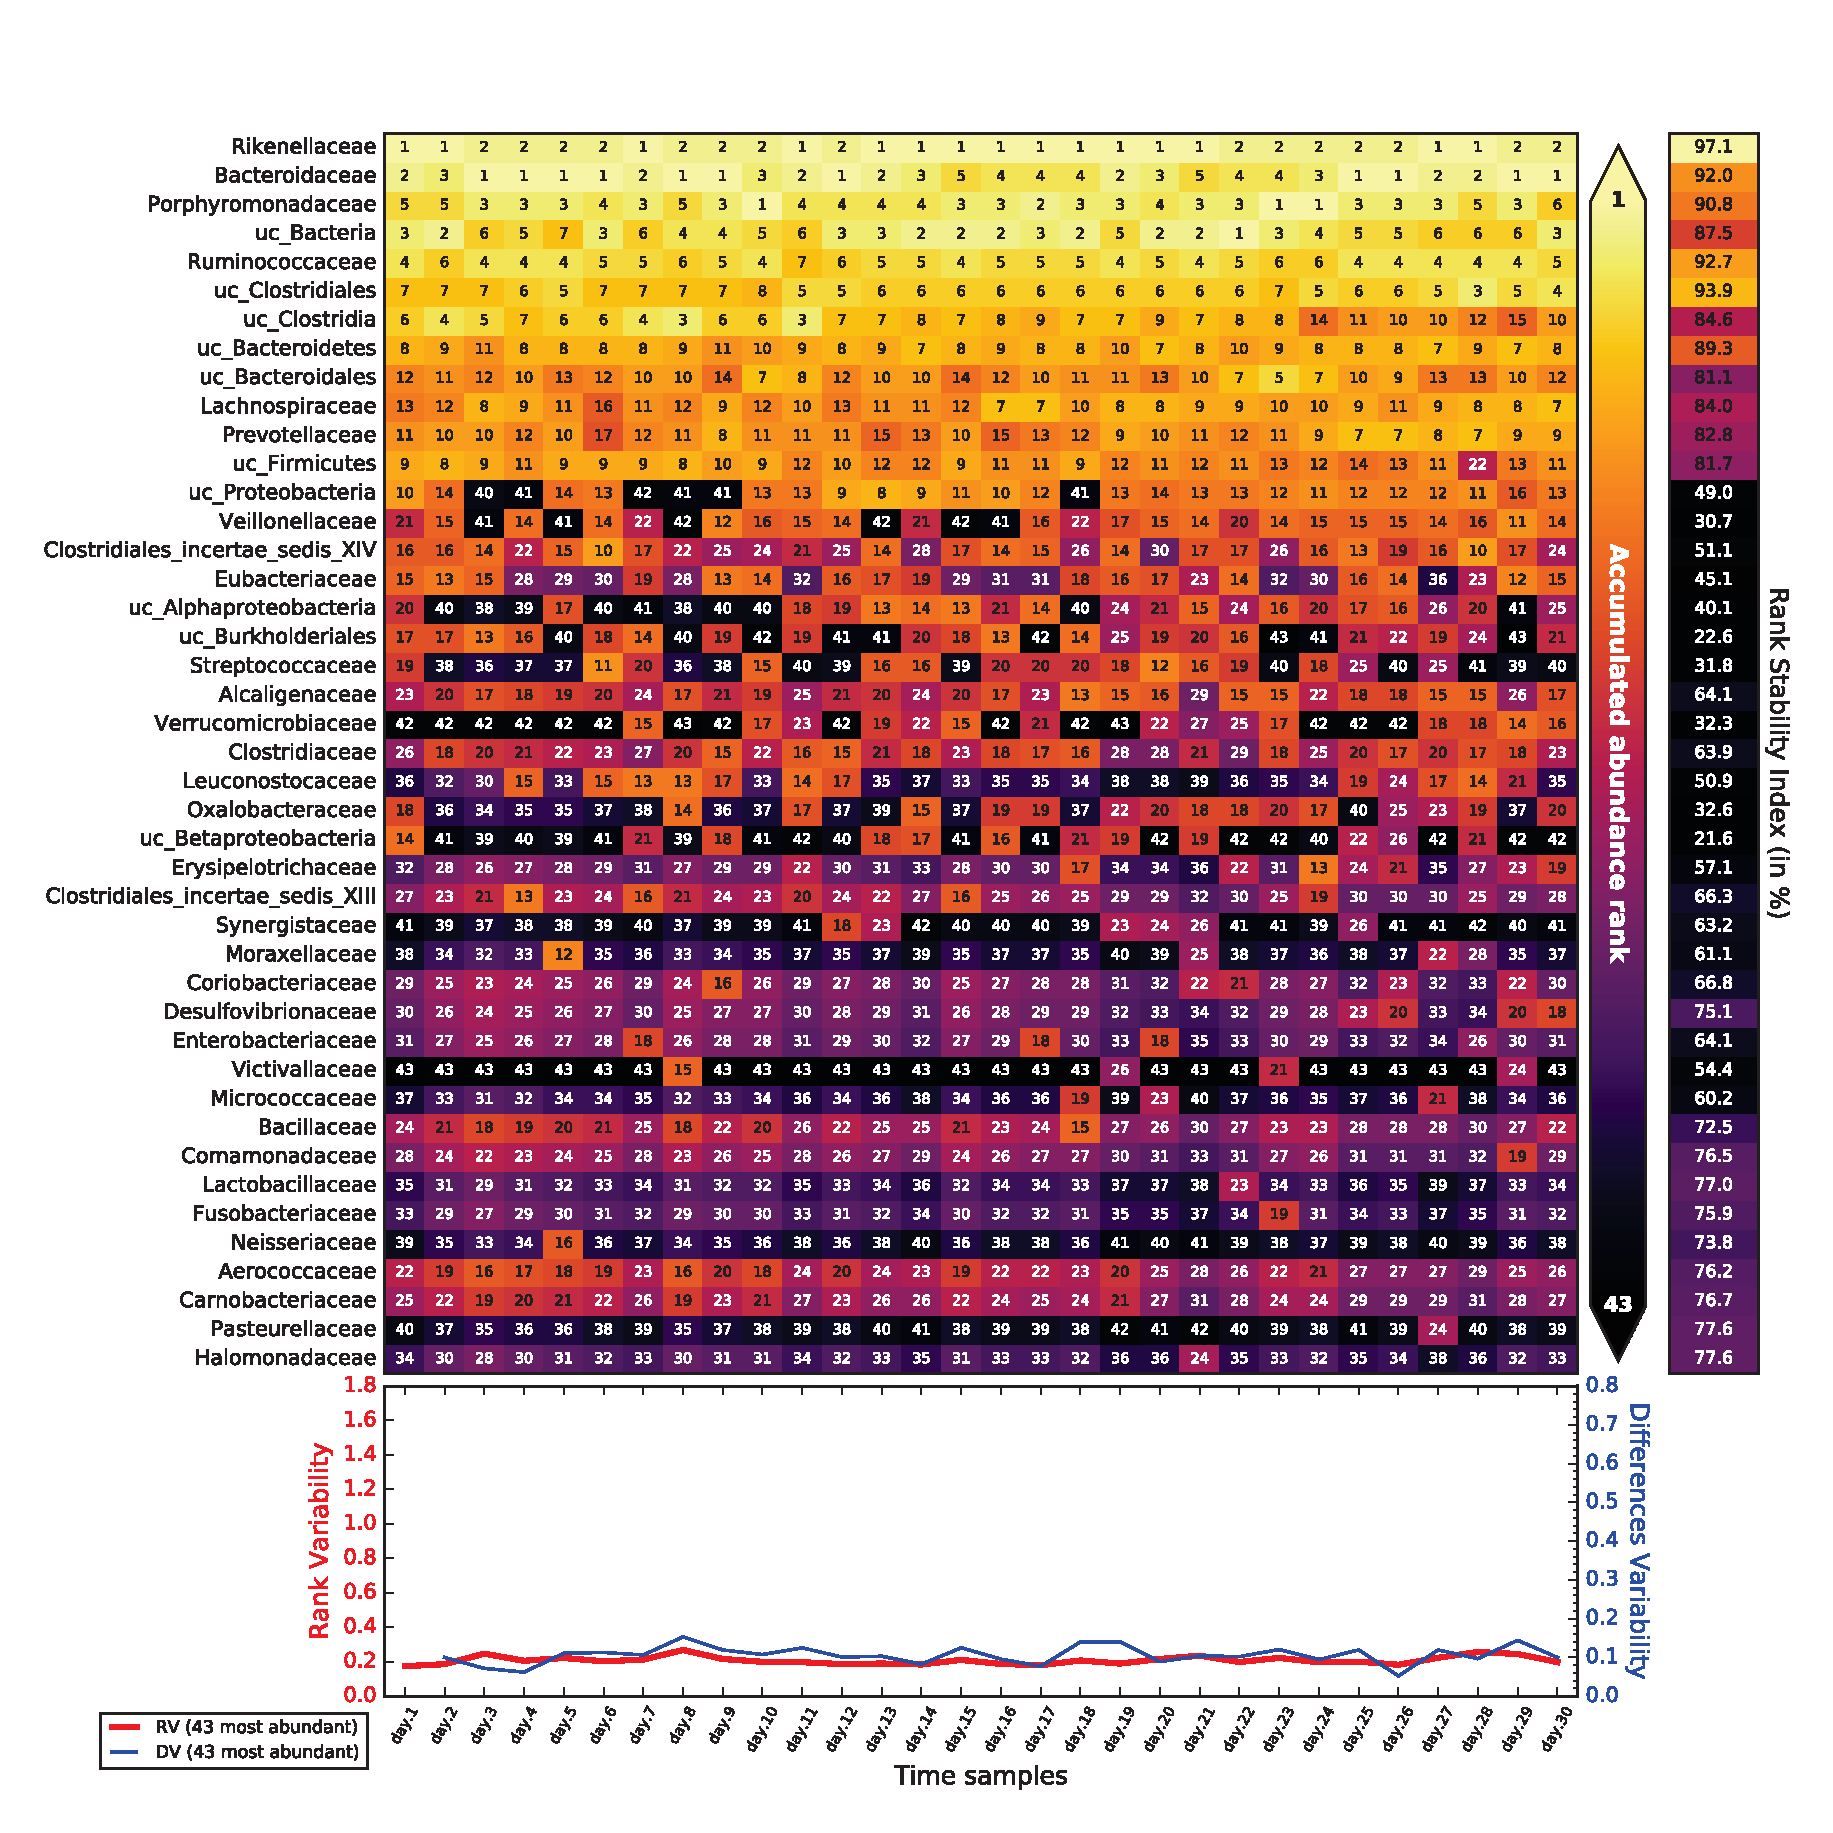
\includegraphics[width=1.0\textwidth]{figs/Fig4.eps}
	\caption{Rank variation over time for the 50 most dominant elements (taxa) and their calculated Rank Stability Index (as shown in Material and Methods) for a special period (days 72 to 122, travelling abroad) belonging to the individual \emph{A} in the host lifestyle study \cite{hostlife}.}
	\label{fig:corrank_HLS_abroad}
\end{figure}

\begin{figure}
	\centering
	%\vspace*{-10mm} % Corrects overbox of the figures \hspace*{-4.5mm}
	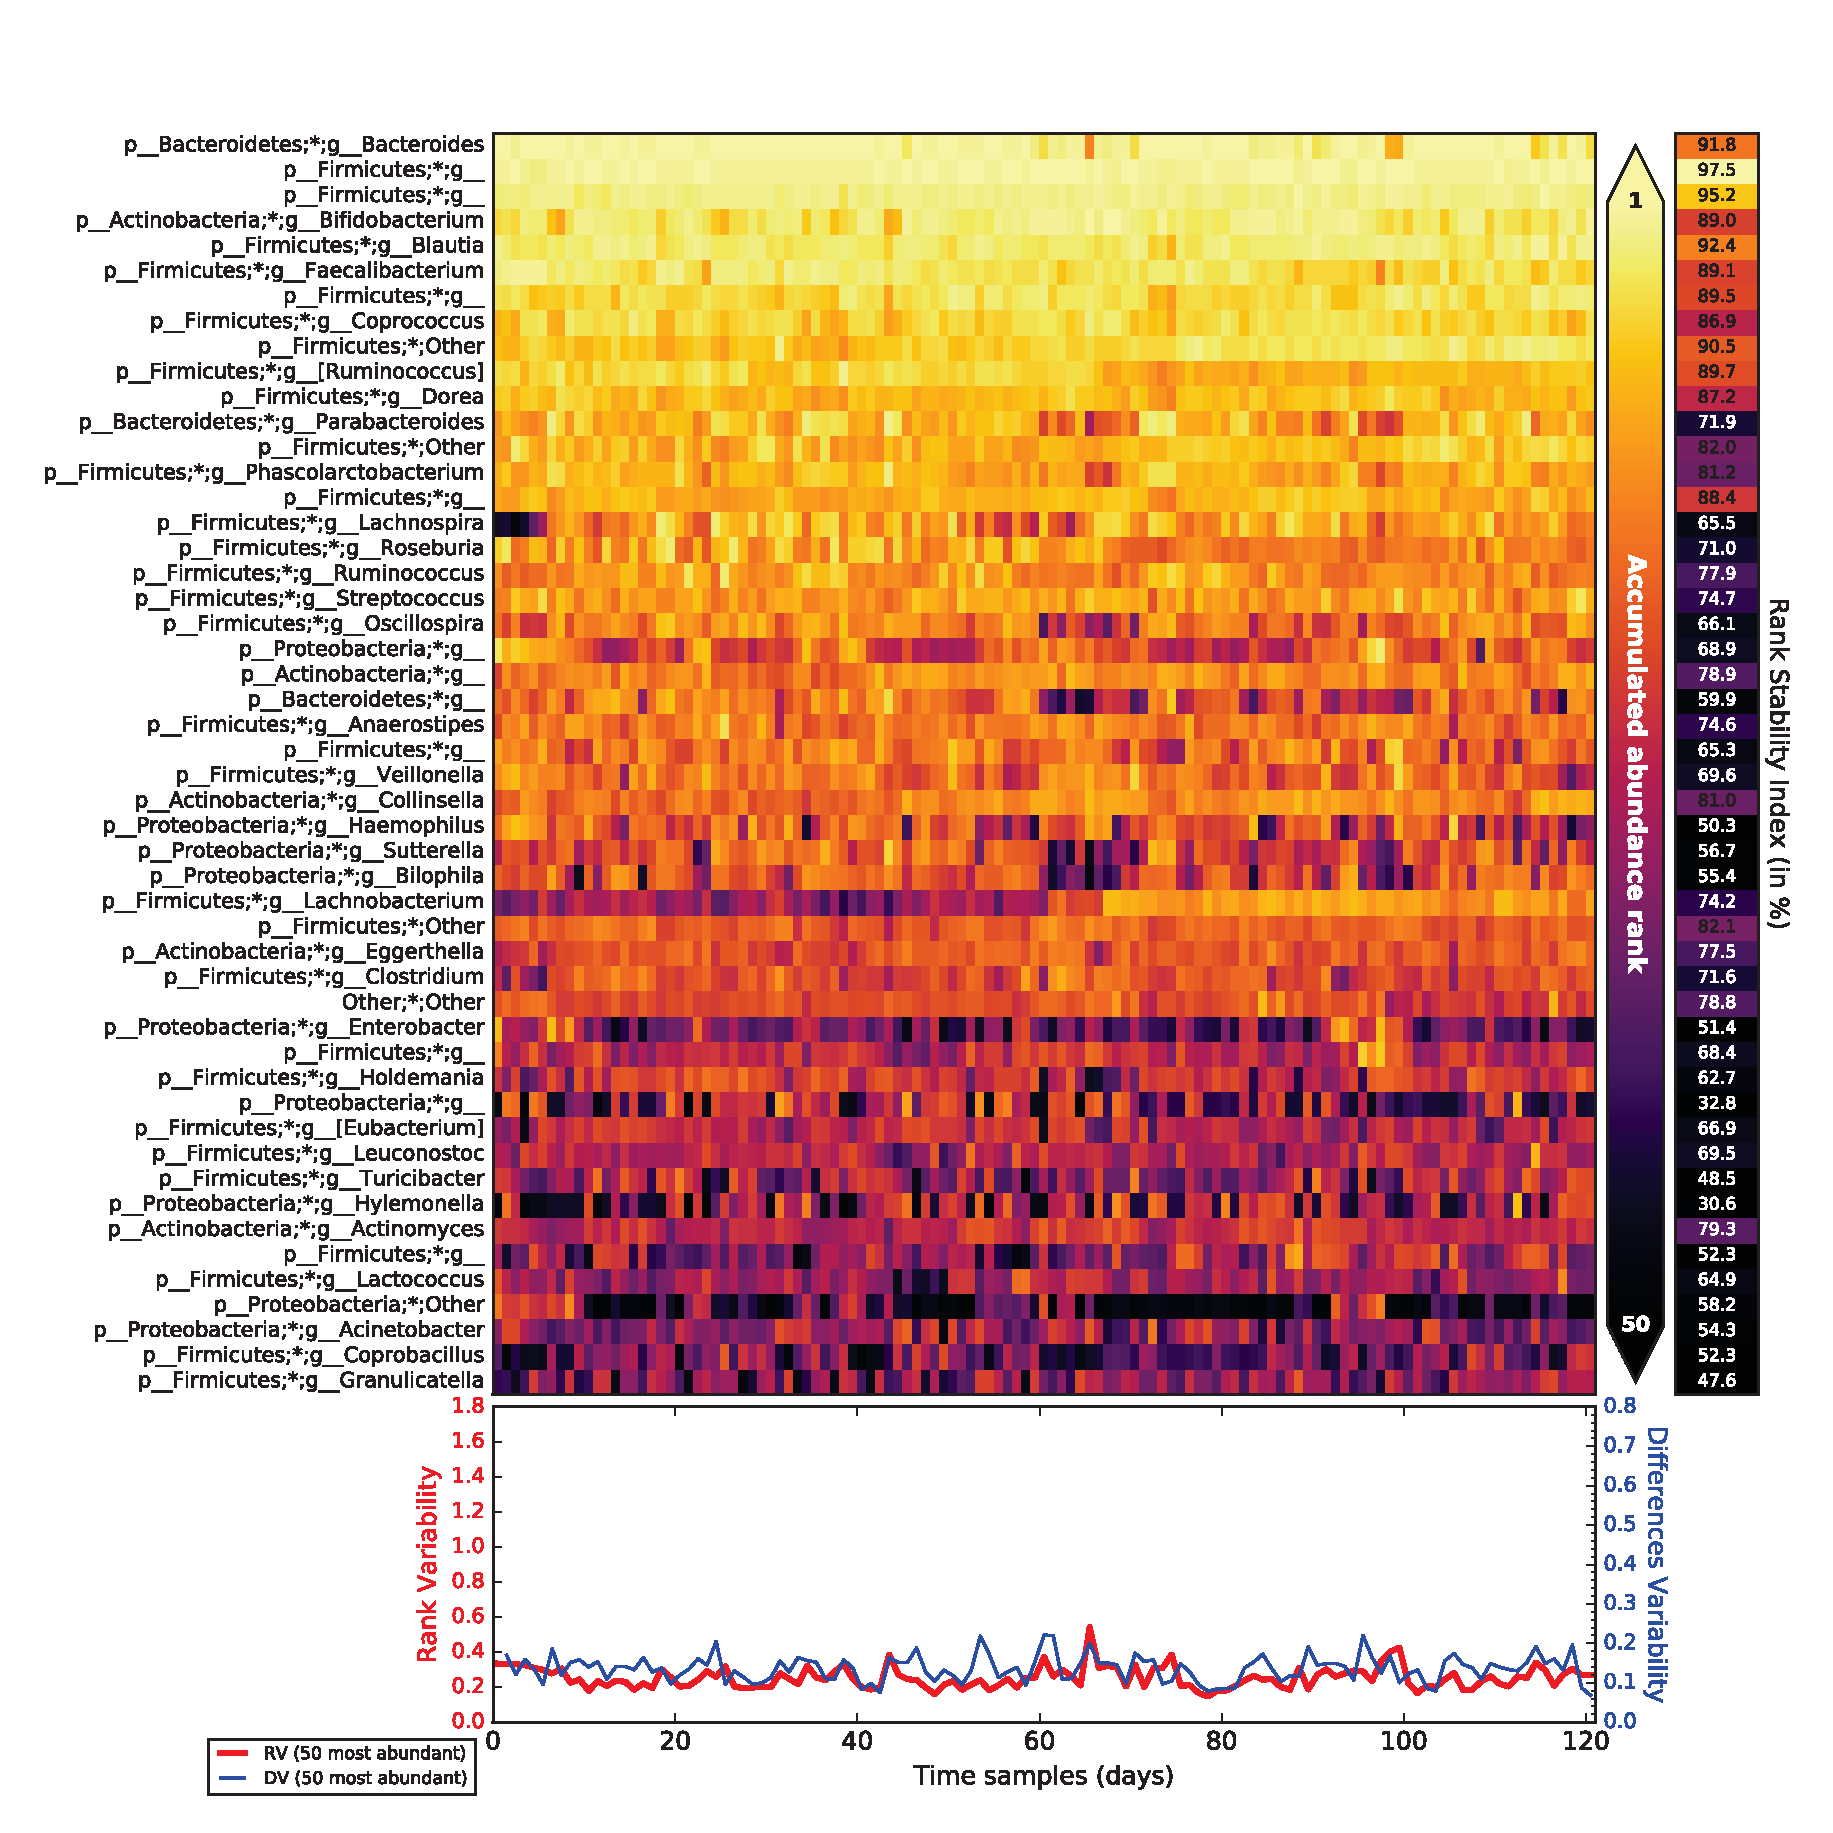
\includegraphics[width=1.0\textwidth]{figs/Fig5.eps}
	\caption{Rank variation over time for the 50 most dominant elements (taxa) and their calculated Rank Stability Index (as shown in Material and Methods) for an ordinary period (days 123 to 256, after the trip) belonging to the individual \emph{A} in the host lifestyle study \cite{hostlife}.}
	\label{fig:corrank_HLS_returned}
\end{figure}

For the trip abroad in Figure \ref{fig:corrank_HLS_abroad}, beyond the differences in dominance for the particular taxa, we still observed that the most dominant were the most rank stable. Moreover, the medium-ranked taxa were quite rank unstable, mostly due to transient (often one or two consecutive samples) yet dramatic drops in their relative abundance, which usually occurred more than twice during their time series.

Nevertheless, in the particular case of the next period, the one subsequent to the trip, in Figure \ref{fig:corrank_HLS_returned}, some taxa showed higher stability than other more dominant taxa, forming a kind of \emph{rank stability islands} for medium--ranked taxa, since they show a moderately stable index (RSI roughly over 70\%). In particular, this is the case for the genera \emph{Actinomyces}, \emph{Leuconostoc}, \emph{Lachnobacterium}, \emph{Eggerthella}, \emph{Clostridium} and	\emph{Collinsella}. For those genera, both the overall rank and the RSI were clearly lower during the trip (RSI under 70\%). \emph{Actinomyces} and \emph{Lachnobacterium} are even not shown in Figure \ref{fig:corrank_HLS_abroad} because they sank to positions 56 and 77, respectively. On the contrary, \emph{Leuconostoc} was the least sensitive to the change of lifestyle. In addition, it is worth mentioning that \emph{Lachnobacterium} showed anti-correlation over time against the vast majority of the taxa classified in this study.

We also found those \emph{rank stability islands} for medium-ranked taxa in the other periods belonging to the individual \emph{A} in the host lifestyle study \cite{hostlife} (see Supplementary Figure S\ref{supfig:corrank_HLS_before} and Supplementary Figure S\ref{supfig:corrank_HLS_after} for the corresponding rank plots). See Supplementary Table S\ref{tab:HLS_RSI} for details about the rank and RSI for the above-mentioned taxa over the different periods considered.

\begin{supfig}
	\centering
	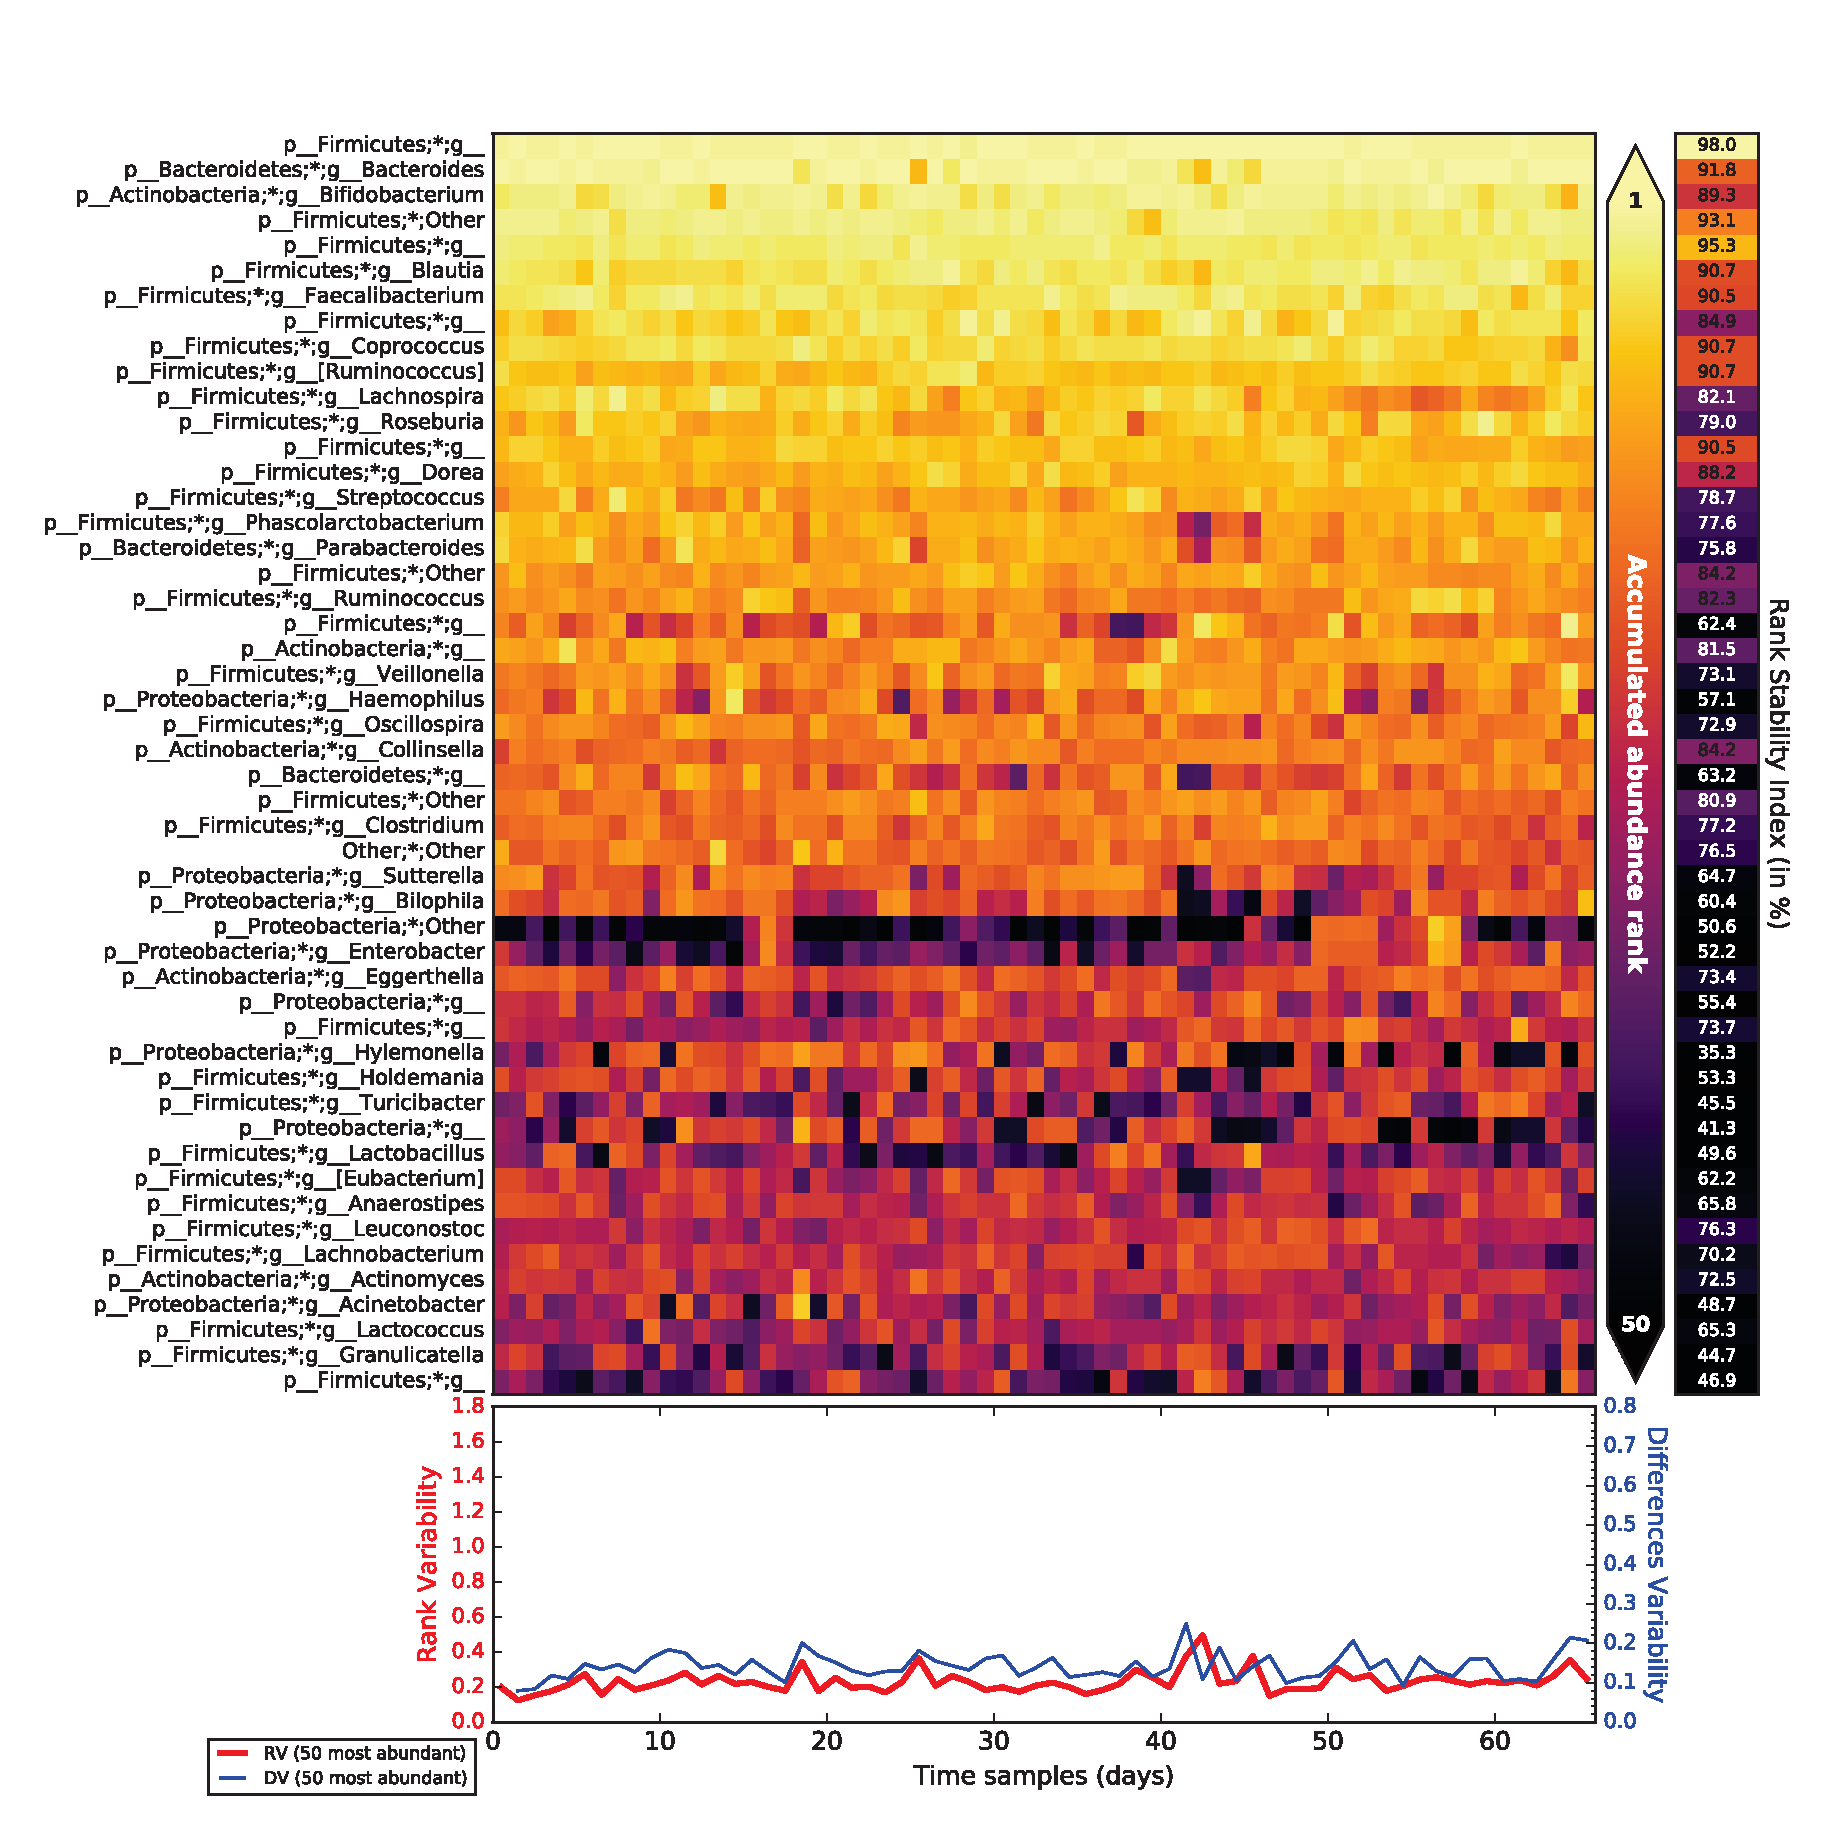
\includegraphics[width=1.0\textwidth]{figs/supfig_corrank_HLS_StoolA_before.eps}
	\caption{Rank variation over time for the 50 most dominant elements (taxa) and their calculated Rank Stability Index (as shown in Material and Methods) for an ordinary period (days 0 to 70, before the trip) belonging to the individual \emph{A} in the host lifestyle study \cite{hostlife}.}
	\label{supfig:corrank_HLS_before}
\end{supfig}

\begin{supfig}
	\centering
	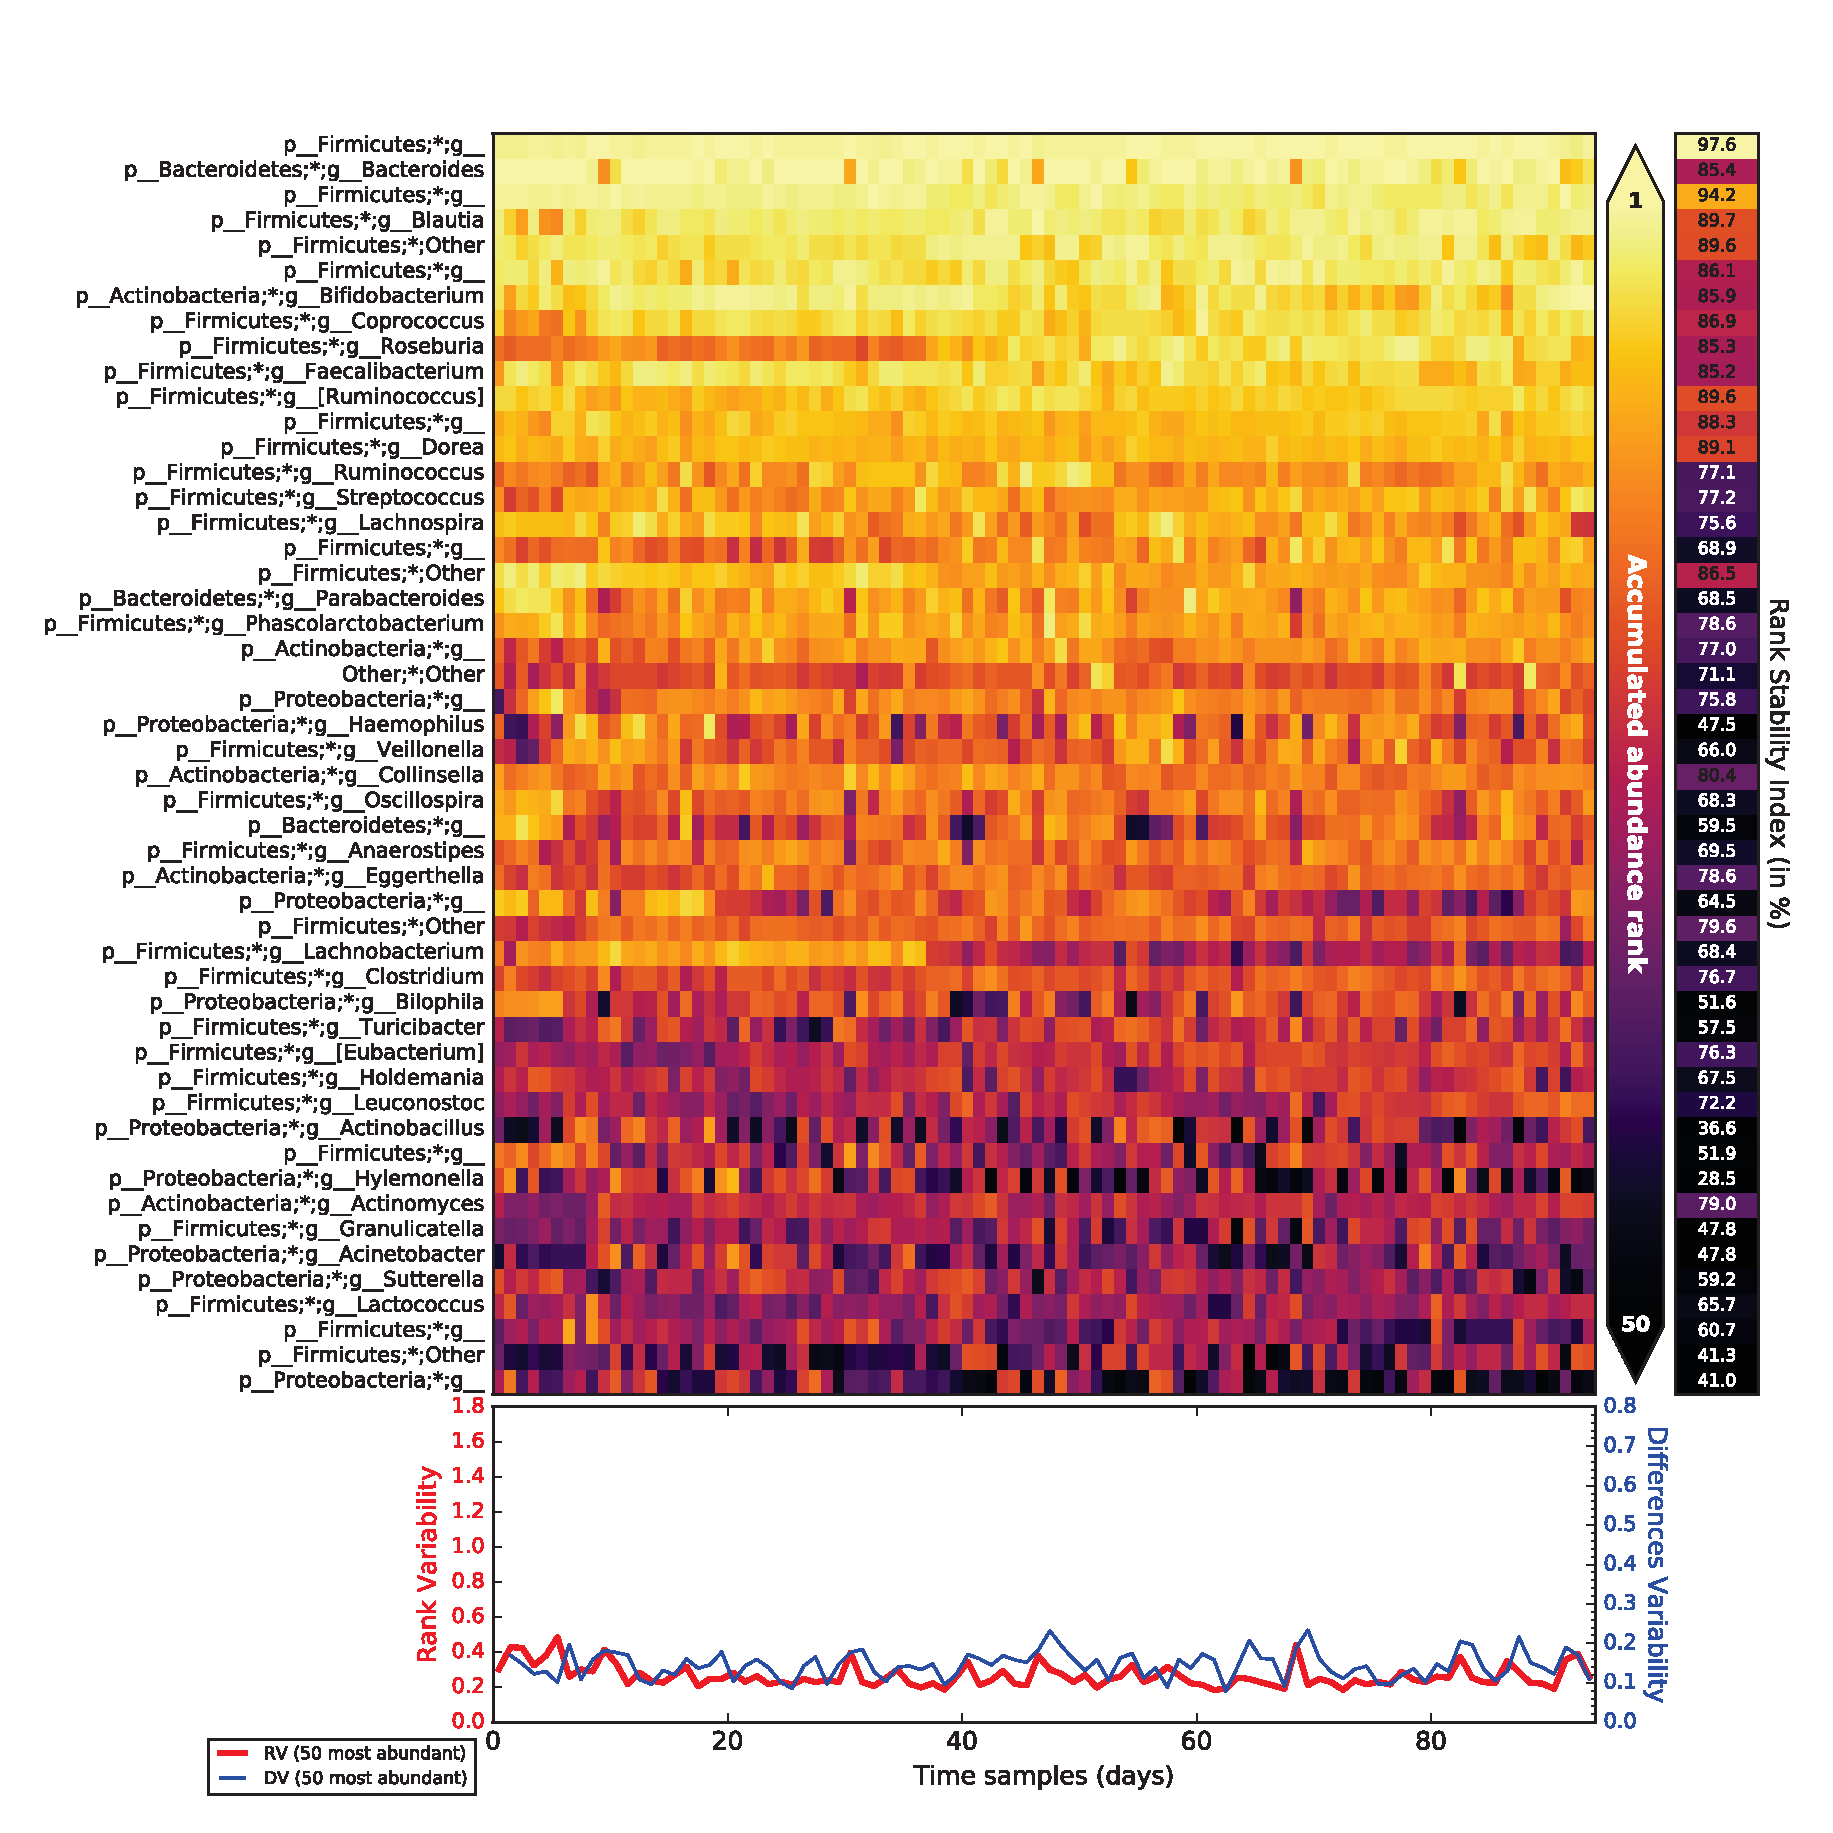
\includegraphics[width=1.0\textwidth]{figs/supfig_corrank_HLS_StoolA_after.eps}
	\caption{Rank variation over time for the 50 most dominant elements (taxa) and their calculated Rank Stability Index (as shown in Material and Methods) for an ordinary period (days 257 to 364, further after the trip) belonging to the individual \emph{A} in the host lifestyle study \cite{hostlife}.}
	\label{supfig:corrank_HLS_after}
\end{supfig}

%%%
\subsection*{Time dependence of model parameters}

Finally, we studied the time dependence of the variability $V$ and power law index $\beta$ (see Model in Material and Methods) by using a sliding window approach. The total number of time points was divided into subsets of five points, where the following subset was defined by adding the next time sampling and eliminating the earliest one. Both parameters were calculated for each subset against the average time lapse. Figure \ref{fig:tempevo1} shows the variability $V$ as a function of time for the largest sampling: two individuals in Caporaso's study\cite{moving} corresponding to the gut microbiota of a male (upper plot) and a female (lower plot). Both samples showed changes in the variability $V$ with quasi--periodic behavior peaking at about 10 days. Variability grew more for the gut microbiota of the male and shared a minimal value of around 0.1 with the gut microbiota of the female. 

Figure \ref{fig:tempevo2} shows the time evolution of $V$ for patient \emph{P2} in the IBS study\cite{IBS} (upper plot) and patient \emph{D} in the antibiotics study\cite{antibiotic} (lower plot). The variability of the gut microbiota of \emph{P2} decreased from over 0.3 to below 0.2, showing a slow tendency to increase the order of the system.  Antibiotic intake led to a quick increase in variability which lasted for a few days to recover ordering. The second antibiotic treatment showed some memory traits (lower increase of variability) with a slower recovery.

\begin{figure}
	%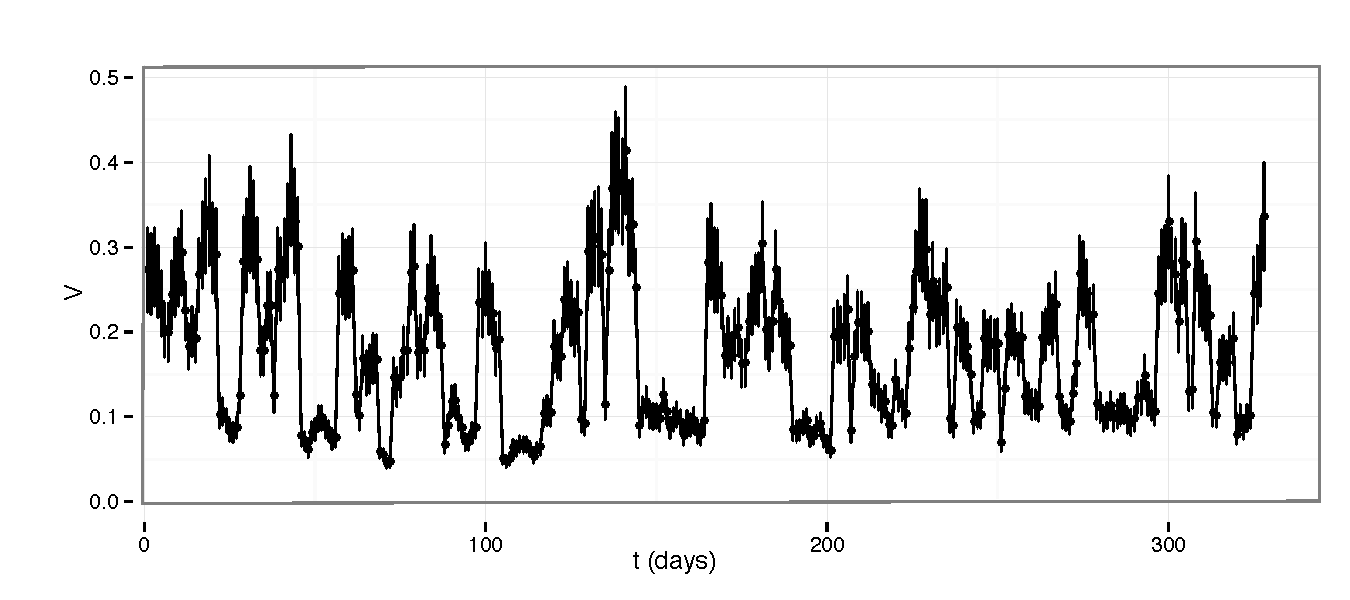
\includegraphics[width=1.0\textwidth]{results/sliwin/male_mov.pdf}
	%\hspace*{3mm}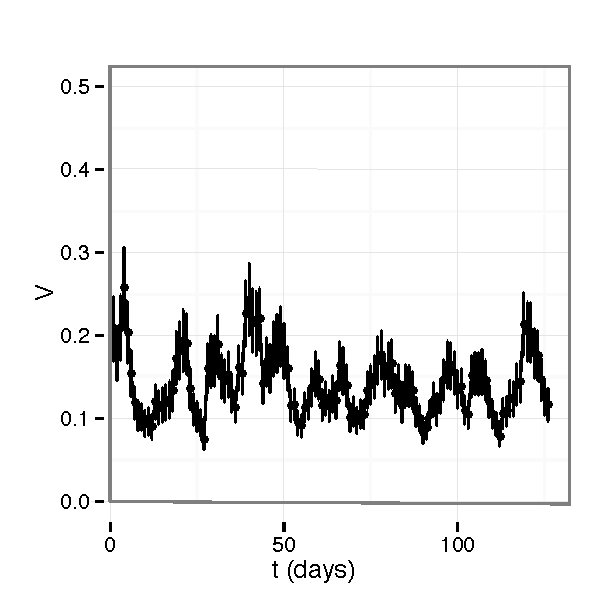
\includegraphics[width=0.448\textwidth]{results/sliwin/female_mov.pdf}
	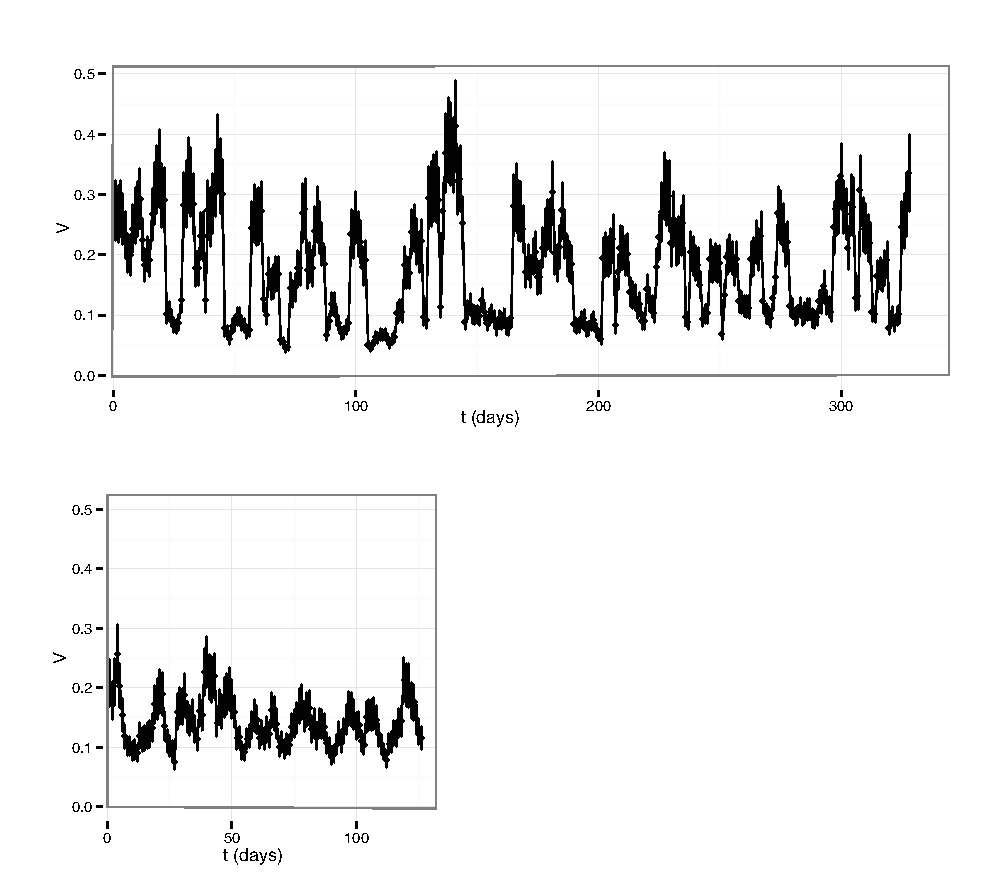
\includegraphics[width=0.99\textwidth]{figs/Fig6.eps}
\caption{$V$ as a function of time for the two individuals in Caporaso's study\cite{moving}: samples of gut microbiome of a male (upper plot) and a female (lower plot).}
\label{fig:tempevo1}
\end{figure}

\begin{figure}
	\centering 
 	%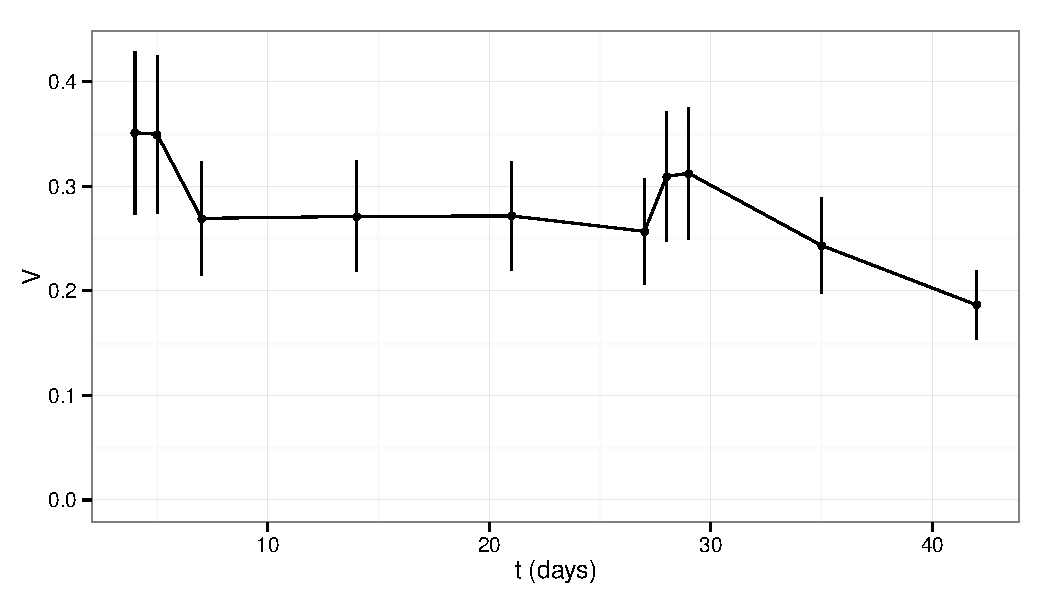
\includegraphics[width=0.8\textwidth]{results/sliwin/patP2_IBS.pdf}
  	%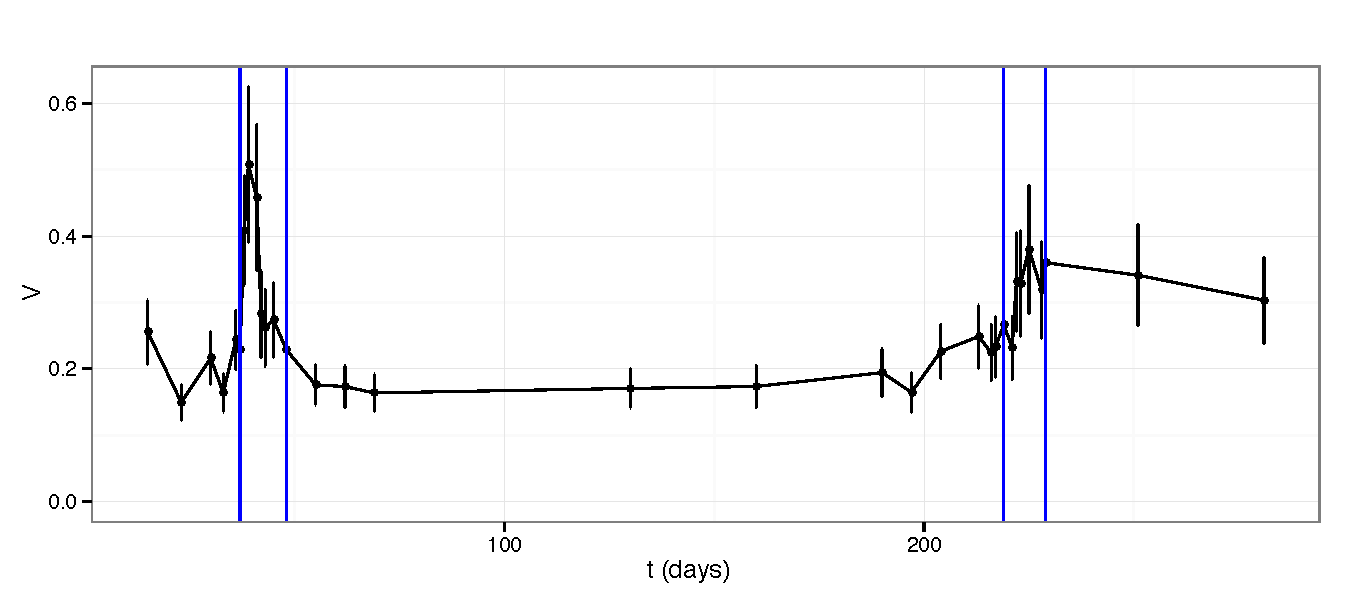
\includegraphics[width=1.0\textwidth]{results/sliwin/patD_antibio.pdf} 
	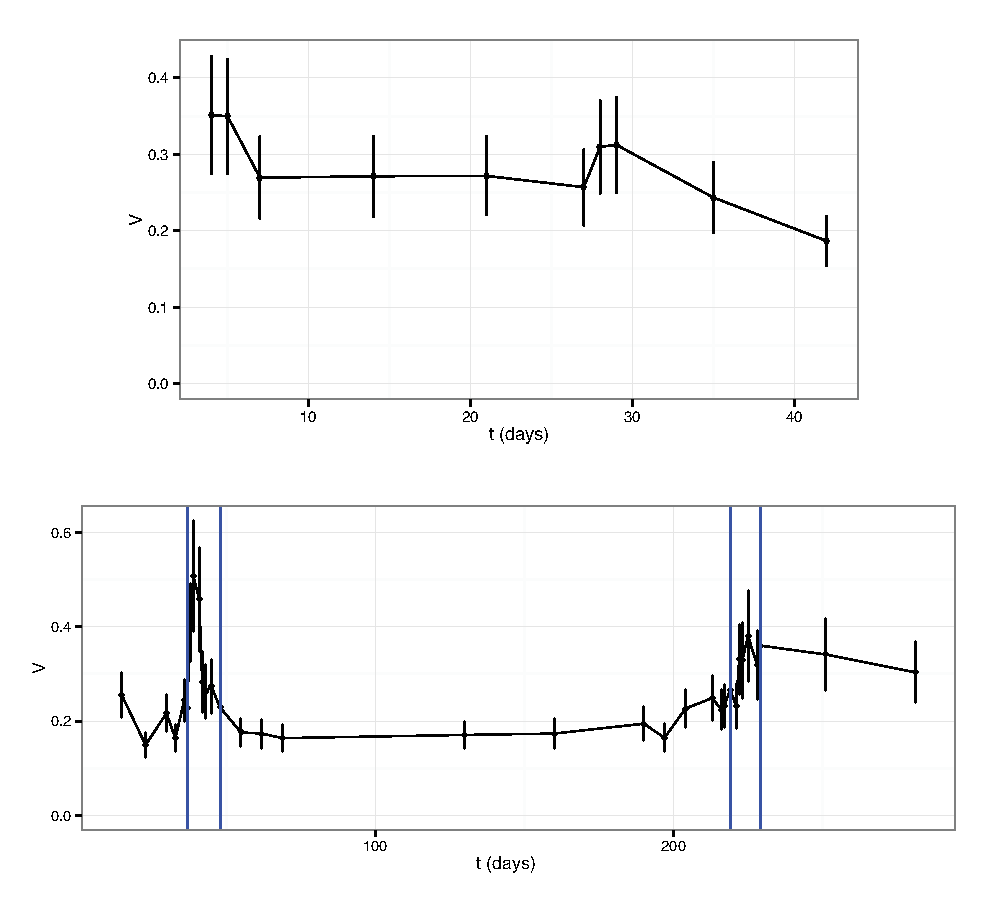
\includegraphics[width=0.99\textwidth]{figs/Fig7.eps}	
\caption{$V$ as a function of time for patient \emph{P2} in the IBS study\cite{IBS} (upper plot) and patient \emph{D} in the antibiotics study\cite{antibiotic} (lower plot). The blue vertical lines in the lower plot show the periods of antibiotic treatment.}
\label{fig:tempevo2}
\end{figure}
